\documentclass [a4paper,final,conference,10pt]{IDAACS}
\usepackage[utf8]{inputenc}
\usepackage[english]{babel}
\usepackage{amsmath}
\usepackage{graphicx}
\usepackage{multirow}
\usepackage{cite}

%\title{Effective Parallelization of Mixed-Critical Software to Distributed Heterogeneous Mutlicoresystems}
%\subtitle{
%	Approaching Challenges of Automotive Constrains: Partial Realtime, Safety, Affinity and Connectivity}
%Bare-Metal and OS-based 
%\title{Constrained Parallelization of Mixed-Critical Applications to Distributed Heterogeneous Hardware}
\title{Constrained Mixed-Critical Parallelization to Distributed Heterogeneous Systems}

\author{
\IEEEauthorblockN{Robert Höttger\IEEEauthorrefmark{1}, Mustafa Özcelikörs\IEEEauthorrefmark{1}}
%						Third Author's Name\IEEEauthorrefmark{2}}

\IEEEauthorblockA{\IEEEauthorrefmark{1}Dortmund University of Applied Sciences and Arts - IDiAL Institute, \\\{robert.hoettger, mustafa.ozcelikors\}@fh-dortmund.de, www.idial.org\\
%						\IEEEauthorrefmark{2}Affiliation, Postal address, e-mail, Web address (URL)\\
%						\IEEEauthorrefmark{3}Affiliation, Postal address, e-mail, Web address (URL)\\
	}
}

\begin{document}
\maketitle

\let\thefootnote\relax\footnotetext{
Identify applicable sponsor/s here. If no sponsors, delete 
this footnote.}

\begin{abstract}
Distributing software effectively to multi-core, many-core, and distributed systems has been studied for decades and still advances successively driven by domain specific constraints. Programming vehicle ECUs (Electronic Constrol Units) is one of the most constrained domains that just recently approached the need for concurrency due to advanced driver assistant systems or autonomous driving approaches. In this paper, various challenges for such systems are outlined, discussed, and solutions are given upon instruction precise modeling, affinity constrained based distribution, and ... The solutions are compared upon bare-metal and OS based implementations while considering fixed priorities for sequential, OS based, and APP4MC scheduling. The latter case has been published at \cite{ICPDSSE} and evolved to consider affinity constraints, SWC-based partitioning and communication cost related mapping. Results show that using APP4MC based distribution on a distributed heterogeneous system outperforms other approaches for mixed-critical applications. %TODO percent

\end{abstract}

\begin{IEEEkeywords}
component; formatting; style; styling
\end{IEEEkeywords}

\section{Introduction}

The automotive domain requires lots of constraints originating from different safety, security, timing, or similar requirements. The verification, validation, testing, and simulation stack requiring dozens of tools, architectures, standards, models, and assessments targets at product-line supporting, consistent, modular, and scalable software but lacks in transparency likewise the comprehensive understanding of applications. Recent approaches already address this challenge and try to provide a common adaptable platform based on AUTOSAR providing a standardized data model. Any specific commercial or proprietary tooling is supposed to be integratable in order to provide seamless interaction with provided tooling such as product-line management, requirements engineering, partitioning, mapping, testing, and more. 
We use the open source APP4MC environment in order to address both industrial and research related models while evaluating our new developments not only regarding model results but also to validate result among a specific use case described in section \ref{sec:rccar}.
The further remainder of this paper is structured as follows: The next section \ref{sec:app4mc} describes modeling 
Section \ref{sec:distribution}
blablablbla 



This template, modified in MS Word 2007 and saved as ``Word 97-2003''
for the PC, provides authors with most of the formatting 
specifications needed for preparing electronic versions of their papers. 
All standard paper components have been specified for 
three reasons: (1) ease of use when formatting individual extended abstract, 
(2) automatic compliance to electronic requirements that facilitate the 
concurrent or later production of electronic products, and (3) conformity of 
style throughout a conference proceedings. Margins, column widths, line 
spacing, and type styles are built-in; examples of the type styles are 
provided throughout this document and are identified in italic type, within 
parentheses, following the example. Some components, such as multi-leveled 
equations, graphics, and tables are not prescribed.

The authors should submit a camera-ready paper of \emph{4~-- 6 pages} 
(in English only) using IDAACS'2015 online submission system. It should 
define \emph{the scope of the work}, emphasize on new advances, 
theories and/or applications and include an analysis of results and findings.
The paper must be structured such that the program committee will 
be able to understand the originality and the value of the work.

\section{Ease of Use}

\subsection{Selecting a Template}

First, confirm that you have the correct template for your paper size. This 
template has been tailored for output on the A4 (210 x 297 mm) paper size. 

In case you prefer the \LaTeX{} please use our slightly modified template 
IDAACS.cls based on the IEEEtran LATEX style and the IEEE bibliography 
template. For details on its usage, please refer to IEEEtran\_HOWTO.pdf.

\subsection{Maintaining the Integrity of the Specifications}

The template is used to format your paper and style the text. All margins,
column widths, line spaces, and text fonts are prescribed; please do not 
alter them. You may note peculiarities. For example, the head margin in 
this template measures proportionately more than is customary. This 
measurement and others are deliberate, using specifications that anticipate
your paper as one part of the entire proceedings, and not as an independent
document. Please do not revise any of the current designations.

\section{Prepare Your Paper Before Styling}

Before you begin to format your paper, first write and save the content as a 
separate text file. Keep your text and graphic files separate until after the
text has been formatted and styled. Do not use hard tabs, and limit use of 
hard returns to only one return at the end of a paragraph. Do not add any 
kind of pagination anywhere in the paper. Do not number text heads-the 
template will do that for you.

Finally, complete content and organizational editing before formatting. 
Please take note of the following items when proofreading spelling and 
grammar:

\subsection{Paper Title}
In the paper title, capitalize the first letter of the first and 
last word and all the nouns, pronouns, adjectives, verbs, adverbs, 
and subordinating conjunctions (\textit{If, Because, That, Which}). 
Capitalize abbreviations that are otherwise lowercase (e.g., use DC, not dc or 
Dc) except for unit abbreviations and acronyms. Articles (\textit{a, an, the}),
coordinating conjunctions (\textit{and, but, for, or, nor}), and most short 
prepositions are lowercase unless they are the first or last word. Prepositions
of more than three letters (\textit{Before, Through, With, Without, Versus, 
Among, Under, Between}) should be capitalized.

\subsection{Abbreviations and Acronyms}

Define abbreviations and acronyms the first time they are used in the text, 
even after they have been defined in the abstract. Abbreviations such as 
IEEE, SI, MKS, CGS, sc, dc, and rms do not have to be defined. Do not use 
abbreviations in the title or heads unless they are unavoidable.

\subsection{Units}
\begin{itemize}
\item {Use either SI (MKS) or CGS as primary units. (SI units are 
encouraged.) English units may be used as secondary units (in parentheses).
An exception would be the use of English units as identifiers in trade, 
such as ``3.5-inch disk drive''.}
\item {Avoid combining SI and CGS units, such as current in amperes and 
magnetic field in oersteds. This often leads to confusion because equations
do not balance dimensionally. If you must use mixed units, clearly state the
units for each quantity that you use in an equation.}
\item {Do not mix complete spellings and abbreviations of units: 
``Wb/m\textsuperscript{2}'' or ``webers per square meter'', not 
``webers/m\textsuperscript{2}''.  Spell out units when they appear in 
text: ``\ldots{} a few henries'', not ``\ldots{} a few H''.}
\item {Use a zero before decimal points: ``0.25'', not ``.25''. Use 
``cm\textsuperscript{3}'', not ``cc''.}
\end{itemize}

\subsection{Equations}

Number equations consecutively with equation numbers in parentheses flush 
with the right margin, as in~(\ref{Eq_1}). To make your equations more compact,
you may use the solidus ( / ), the exp function, or appropriate exponents. 
Italicize Roman symbols for quantities and variables, but not Greek symbols.
Use an en dash (--) rather than a hyphen for a minus sign. Use parentheses to
avoid ambiguities in denominators. 

\begin{equation}
\label{Eq_1}
\lambda_i = \lim \frac{1}{p} \sum_{t=1}^p \ln \frac{|w_i (t)|}{|w_i (t-1)|}
\end{equation}

Please set in Microsoft Equation following fonts: Regular~--- 12~pt, Large 
index~--- 7~pt, Small index~--- 5~pt, Large symbol~--- 18~pt, Small 
Symbol~--- 12~pt.

Note that the equation is centered using a center tab stop. Be sure that the
symbols in your equation have been defined before or immediately following 
the equation. Use ``~(\ref{Eq_1})'', not ``Eq.~(\ref{Eq_1})''or 
``equation~(\ref{Eq_1})'', except at the beginning of a sentence: 
``Equation~(\ref{Eq_1}) is \ldots{}''.

\subsection{Some Common Mistakes}

\begin{itemize}
\item {The word ``data'' is plural, not singular.}
\item {The subscript for the permeability of vacuum $\mu_0$, and other 
common scientific constants, is zero with subscript formatting, not a 
lowercase letter ``o''.}
\item {In American English, commas, semi-colons, periods, question and
exclamation marks are located within quotation marks only when a complete
thought or name is cited, such as a title or full quotation. When quotation
marks are used, instead of a bold or italic typeface, to highlight a word 
or phrase, punctuation should appear outside of the quotation marks. 
A parenthetical phrase or statement at the end of a sentence is punctuated 
outside of the closing parenthesis (like this). (A parenthetical sentence 
is punctuated within the parentheses.)}
\item{A graph within a graph is an ``inset'', not an ``insert''. The word 
alternatively is preferred to the word ``alternately'' (unless you really 
mean something that alternates).}
\item{Do not use the word ``essentially'' to mean ``approximately'' or 
``effectively''.}
\item{In your paper title, if the words ``that uses'' can accurately replace 
the word ``using'', capitalize the ``u''; if not, keep using lower-cased.}
\item{Be aware of the different meanings of the homophones ``affect'' and 
``effect'', ``complement'' and ``compliment'', ``discreet'' and ``discrete'',
``principal'' and ``principle''.}
\item{Do not confuse ``imply'' and ``infer''.}
\item{The prefix ``non'' is not a word; it should be joined to the word it 
modifies, usually without a hyphen.}
\item{There is no period after the ``et''” in the Latin abbreviation 
``et al.''.}
\item{The abbreviation ``i.e.'' means ``that is'', and the abbreviation 
``e.g.'' means ``for example''.}
\end{itemize}

An excellent style manual for science writers is~\cite{publ7}.

\section{Using the Template}

After the text edit has been completed, the paper is ready for the 
template. Duplicate the template file by using the Save As command, and use 
the naming convention prescribed by your conference for the name of your 
paper. In this newly created file, highlight all of the contents 
and import your prepared text file. You are now ready to style your paper; 
use the scroll down window on the left of the MS Word Formatting toolbar.

Type the text of the paper in two columns. Balance the length of 
the columns, especially on the last page of the paper. Left- and 
right-justify your columns. Use tables and figures to adjust column length. 
On the last page of your paper, adjust the lengths of the columns 
so that they are equal. Use automatic hyphenation and check spelling. 
Digitize or paste down figures.

\subsection{Authors and Affiliations}

The template is designed so that author affiliation are not repeated each time
for multiple authors of the same affiliation. Please keep your affiliation in
as succinct as possible (for example, do not differentiate among departments
of the same organization).

\subsection{Identify the Headings}

Headings, or heads, are organizational devices that guide the reader through 
your paper. There are two types: component heads and text heads.

Component heads identify the different components of your paper and are not 
topically subordinate to each other. Examples include Acknowledgments and 
References and, for these, the correct style to use is ``Heading 5''. Use 
``figure caption'' for your Figure captions, and ``table head'' for your 
table title. Run-in heads, such as ``Abstract'', will require you to apply a 
style (in this case, italic) in addition to the style provided by the drop 
down menu to differentiate the head from the text.

Text heads organize the topics on a relational, hierarchical basis. For 
example, the paper title is the primary text head because all subsequent 
material relates and elaborates on this one topic. If there are two or 
more sub-topics, the next level head (uppercase Roman numerals) should be 
used and, conversely, if there are not at least two sub-topics, then no 
subheads should be introduced. Styles named ``Heading 1'', ``Heading 2'',
``Heading 3'', and ``Heading 4'' are prescribed.

\subsection{Positioning Figures and Tables}

Place figures and tables after they are first cited in the text. Large 
figures and tables may span across both columns. Figure captions should 
be centered below the figures; table heads should appear above the tables. 
Use the abbreviation ``Fig.~\ref{Fig_Magnet}'', even at the beginning of a 
sentence.

\begin{figure}[bth]
\centering
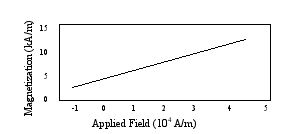
\includegraphics[scale=0.6]{images/Fig1.png}
\caption{\label{Fig_Magnet}Magnetization as a function of applied field. Note 
how the caption is centered in the column.}
\end{figure}

\begin{table}[htb]
\caption{Table Type Styles}
\label{Table_I}
\centering
\begin{tabular}{|p{1.2cm}|p{1.5cm}|p{1.5cm}|p{1.5cm}|}
\hline
\multirow{2}{1.2cm}{\textbf{Type Size (pts.)}} & \multicolumn{3}{|c|}{\textbf{Appearance}}\\
\cline{2-4}
& \textbf{\textit{Regular}}&\textbf{\textit{Bold}}&\textbf{\textit{Italic}}\\
\hline
8 & References, table header, footnotes, text subscripts, and superscripts &&\\
\hline
9 & Table captions and table names - uppercase. Table superscripts, 
figure captions.& Abstract, keywords& Words ``Abstract'' and ``Keywords''\\
\hline 
10 & Authors' affiliations, main text, equations && Subheadings\\
\hline
11 & Authors' names &&\\
\hline
20 & Paper title &&\\
\hline
\end{tabular}
\end{table}

We suggest that you use a table to insert a graphic (which is ideally a 300 dpi
TIFF or EPS file, with all fonts embedded) and it’s caption, because, in an MSW
document, this method is somewhat more stable than directly inserting a picture.

Figure Labels: Use 8 point Times New Roman for Figure labels. Use words rather
than symbols or abbreviations when writing Figure axis labels to avoid 
confusing the reader. As an example, write the quantity ``Magnetization'', or 
``Magnetization, M'', not just ``M''. If including units in the label, present
them within parentheses. Do not label axes only with units. In the example, 
write ``Magnetization (A/m)'' or ``Magnetization {A[m(1)]}'', not just ``A/m''.
Do not label axes with a ratio of quantities and units. For example, write 
``Temperature (K)'', not ``Temperature/K''.


\subsection{References}

Number citations consecutively in square brackets~\cite{publ1}.
The sentence punctuation follows the bracket~\cite{publ2}. Refer simply to the
reference number, as in~\cite{publ3}. Do not use ``Ref.~\cite{publ3}'' or 
``reference~\cite{publ3}'' except at the beginning of a sentence: 
``Reference~\cite{publ3} was the first \ldots{}''

Grammatically, they may be treated as if they were footnote numbers, e.g., 
as shown by Clerk Maxwell~\cite{publ2}; as mentioned earlier~\cite{publ7, 
publ2, publ3, publ4, publ6}; Jacobs and Bean~\cite{publ5}; Yorozu et 
al~\cite{publ6}.

Number footnotes separately in superscripts. Place the actual footnote at the 
bottom of the column in which it was cited. Do not put footnotes in the 
reference list. Use letters for table footnotes.

Unless there are six authors or more give all authors' names; do not use 
``et al.''. Papers that have not been published, even if they have been 
submitted for publication, should be cited as ``unpublished''~\cite{publ4}. 
Papers that have been accepted for publication should be cited as 
``in press''~\cite{publ5}. Capitalize only the first word in a paper title, 
except for proper nouns and element symbols.

For papers published in translation journals, please give the English citation 
first, followed by the original foreign-language citation~\cite{publ6}. If 
paper was published in other than English, please translate it and provide
original-language title in round brackets, like in~\cite{publ8}.

\section*{Acknowledgment}
References and Acknowledgment headings are not enumerated. They are simply 
primary headings without labels, regardless of whether the other headings 
in the papers are enumerated.

The placement of the Acknowledgment appears after the final text of the 
paper, just before the References section, and after any Appendix(es).

All acknowledgment of financial support must be removed from the 
Acknowledgment section, and placed in the first paragraph of the first 
footnote.

Write the Acknowledgment section to be read in the third person.
\enlargethispage{-7in}
The preferred spelling of the word ``acknowledgment'' in America 
is without an ``e'' after the ``g''. Try to avoid the stilted 
expression, ``One of us (R. B. G.) thanks \ldots''. Instead, 
try ``R.B.G. thanks \ldots{}''. 

When citing names within the Acknowledgment, use first initials 
only, not full names. Do not use Mr., Mrs., Ms., or Miss 
(list first initial and last name only). Use the Dr. or Prof. 
title with each name separately; do not use plural Drs. or 
Profs. with lists of names.

%Put sponsor acknowledgments 
%in the unnumbered footnote on the first page.

\bibliographystyle{IEEEtran}
\bibliography{IEEEabrv,IDAACS_Example}


\end{document}
